\documentclass[10.5pt
%,draft
]{article}


\usepackage{ctex}
\usepackage{graphicx}
\usepackage{amsmath}
\usepackage{xcolor}
\usepackage{physics}
\usepackage{hyperref}
\hypersetup{
    colorlinks=true,
    linkcolor=Blue4Link,
    filecolor=magenta,      
    urlcolor=cyan,
    pdfauthor=徐均益
    }
\definecolor{Blue4Link}{RGB}{46,49,146}
\definecolor{myOrange}{RGB}{178,76,0}
\definecolor{green4eye}{RGB}{0,120,2}%
\definecolor{blue4eye}{RGB}{1,126,218}%
\definecolor{cyan4eye}{RGB}{31,186,190}%
\definecolor{myhighlight}{RGB}{255,214,161}
\definecolor{mybackground}{RGB}{204,232,207}
\usepackage{geometry}
\usepackage{natbib}
\usepackage{subcaption}
\usepackage{epstopdf}
\usepackage{tikz}
\usepackage{psfrag}
\usepackage{natbib}

\def\due{2023 年 5 月 26 日周五 08:40}
\def\Term{2023 年春季}
\def\Course{磁流体力学的数值模拟方法}

\renewcommand{\refname}{参考文献}
\renewcommand{\figurename}{图}
\renewcommand{\abstractname}{摘要}

\title{一维磁流体力学激波 --- 第 4 次作业\footnote{\Term\Course}}

\author{徐均益\footnote{ID: SA22214015 Email: jyxu@mail.ustc.edu.cn}
  \and
  余航\footnote{ID: SA22168021 Email: yh131996@mail.ustc.edu.cn}
  \and
  陈宇韬\footnote{ID: SA22214014 Email: chenyut@mail.ustc.edu.cn}
}

\date{%
\scriptsize%
%CAS Key Laboratory for Basic Plasma Physics, School of Earth and Space Sciences,
%\\
%University of Science and Technology of China, Hefei, Anhui 230026, China
中国科学技术大学核科学技术学院, 合肥 230026 \\
中国科学技术大学物质科学研究院等离子所, 合肥 230026
%
}

\begin{document}

\maketitle

\begin{abstract}
研究讨论一维磁流体力学 (MHD, Magnetohydrodynamics) 激波问题的有限差分数值解法, 主要采用守恒形式的Lax-Wendroff格式,结合理论分析讨论磁声波的特性,
以及分析数值格式的计算效果。以及其他格式如隐格式和迭代法的相关尝试。
\end{abstract}

\section{引言}
磁流体力学 (MHD, Magnetohydrodynamics) 是磁流体的宏观描述,MHD方程将流体力学,麦克斯韦方程以及洛仑兹力结合起来,是一个多元非线性方程。其对应的MHD模拟是太阳物理里面非常常用的手段,比如磁绳爆发模拟等等。在本次作业中,我们在上次一维气体激波管问题的基础上,添加磁流体力学方程组,对一维磁流体力学激波问题进行模拟和分析。

\section{理论介绍}\label{DLess}
本次我们采用无量纲数值的守恒形式, 将磁流体力学方程表示为
\begin{align}
\frac{\partial U}{\partial t} + \frac{\partial F}{\partial x} = 0 \label{Eqn:MHD}
\end{align}
其中
\begin{align}
U = & \left[ \begin{array}{l}
\rho\\
\rho v^2 + H_y^2 + H_z^2 + \frac{\beta p}{\gamma -1}
\\
\rho v_x\\
\rho v_y\\
\rho v_z\\
H_y\\
H_z
\end{array} \right]\label{Eqn:Flux_U}, \\
F = & \left[ \begin{array}{l}
\rho v_x\\
\rho v_x \left(v^2 + \frac{\gamma}{\gamma - 1} \frac{\beta p}{\rho} \right) + 2(H_y^2 v_x + H_z^2 v_x - H_x H_y v_y - H_x H_z v_z)
\\
\rho v_x^2 + \frac{\beta}{2} p + \frac{1}{2} (H_y^2 + H_z^2)\\
\rho v_x v_y - H_x H_y\\
\rho v_x v_z - H_x H_z\\
v_x H_y - v_y H_x\\
v_x H_z - v_z H_x
\end{array} \right] \label{Eqn:Flux}
\end{align}
这里 $v^2 = v_x^2 + v_y^2 + v_z^2$. 若取 $\rho_0 = 1$, $p_0 = 1$, $v_0 = 1$, $H_0 = 1/\sqrt{4\pi}$, 则 $\beta = 2$,

其中 $A = \frac{\partial F}{\partial u}$, $A$ 的表达式为
\begin{equation}
   \mqty[
0  &  0  &  1  &  0  &  0  &  0  &  0 \\
% (2 H_x \rho (H_y m_y+H_z m_z)+m_x (\rho (-\gamma E +(\gamma-2) H_y^2+(\gamma-2) H_z^2)+2 (\gamma-1) m_y^2+2 (\gamma-1) m_z^2)+2 (\gamma-1) m_x^3)/\rho^3  &  (\gamma m_x)/\rho  &  -((-\gamma E \rho+(\gamma-2) H_y^2 \rho+(\gamma-2) H_z^2 \rho+3 (\gamma-1) m_x^2+(\gamma-1) m_y^2+(\gamma-1) m_z^2)/\rho^2)  &  -((2 (H_x H_y \rho+(\gamma-1) m_x m_y))/\rho^2)  &  -((2 (H_x H_z \rho+(\gamma-1) m_x m_z))/\rho^2)  &  -((2 (H_x m_y+(\gamma-2) H_y m_x))/\rho)  &  -((2 (H_x m_z+(\gamma-2) H_z m_x))/\rho) \\
\dots  &  \dots  &  \dots  &  \dots  &  \dots  &  \dots  &  \dots \\
\frac{(\gamma-1) v^2-2v_x^2}{2 }  &  \frac{\gamma-1}{2}  &  (3-\gamma) v_x  & (1-\gamma) v_y  &  (1-\gamma) v_z  &  (2-\gamma) H_y  &  (2-\gamma) H_z \\
-v_x v_y  &  0  &  v_y  &  v_x  &  0  &  -H_x  &  0 \\
-v_x v_z  &  0  &  v_z  &  0  &  v_x  &  0  &  -H_x \\
\frac{H_x v_y-H_y v_x}{\rho}  &  0  &  \frac{H_y}{\rho}  &  -\frac{H_x}{\rho}  &  0  &  v_x  &  0 \\
H_x v_z-H_z v_x  &  0  &  \frac{H_z}{\rho}  &  0  &  -\frac{H_x}{\rho}  &  0  &  v_x ]
\label{eq:Lax-Wendroff-A}
\end{equation}
矩阵第二行7个元素分别为
\begin{subequations}
	\begin{gather}
% (2 H_x \rho (H_y m_y+H_z m_z)+m_x (\rho (-\gamma E +(\gamma-2) H_y^2+(\gamma-2) H_z^2)+2 (\gamma-1) m_y^2+2 (\gamma-1) m_z^2)+2 (\gamma-1) m_x^3)/\rho^3   \\
-\frac{2 (H_y^2+H_z^2) v_x (1- \gamma) -2 H_x (H_y v_y+H_z v_z )(1 - \gamma) - p v_x \beta \gamma + v_x v^2 (2 - 3 \gamma + \gamma^2) \rho}{(1 - \gamma) \rho}\\
  \gamma v_x   \\
  -((-\gamma E \rho+(\gamma-2) H_y^2 \rho+(\gamma-2) H_z^2 \rho+3 (\gamma-1) m_x^2+(\gamma-1) m_y^2+(\gamma-1) m_z^2)/\rho^2)   \\
  -((2 (H_x H_y \rho+(\gamma-1) m_x m_y))/\rho^2)   \\
  -((2 (H_x H_z \rho+(\gamma-1) m_x m_z))/\rho^2)   \\
  -((2 (H_x m_y+(\gamma-2) H_y m_x))/\rho)   \\
  -((2 (H_x m_z+(\gamma-2) H_z m_x))/\rho) 
\end{gather}
\end{subequations}
其中
$ m_x = \rho v_x,
m_y = \rho v_y,
m_z = \rho v_z.$
\section{数值格式介绍}
本次实验我们尝试设计多种格式: Upwind, Lax-Wendroff, TVD,实现了两支间断较小的激波的模拟,其中 Upwind 和 TVD 较为稳定。
\subsection{数值实验设计}

考虑下列初值问题
\begin{align}
U(x,t)|_{t=0} = \left\{ \begin{array}{ll}
U_L, & \quad x < x_0 \\
U_R, & \quad x > x_0
\end{array} \right.
\end{align}
或者
\begin{align}
W(x,t)|_{t=0} = \left\{ \begin{array}{ll}
W_L, & \quad x < x_0 \\
W_R, & \quad x > x_0
\end{array} \right.
\end{align}
的有限差分数值计算. 这里 $U$ 的表达式由方程~(\ref{Eqn:Flux_U}) 给出, 具体实验时需要将$W$转化成$U$,然后再代入数值程序中进行计算。
\begin{align}
W = \left[ \begin{array}{ccccccc}
\rho,
p,
v_x,
v_y,
v_z,
H_y,
H_z
\end{array} \right]^T.
\end{align}
上标 $T$ 表示转置操作. 取 $\gamma=5/3$, $\mu=1$, $H_x=5$. 分别就如下初值条件设计实验

\subsubsection{较弱的快激波}
取 $x_0 = 0.0$, 快激波条件为
\begin{align}
W_L &= \left[\begin{array}{cccccc}
2.121,
4.981,
-13.27,
-0.163,
-0.6521,
2.572,
10.29
\end{array}\right]^T,
\nonumber\\
W_R &= \left[\begin{array}{ccccccc}
1,
1,
-15.3,
0,
0,
1,
4
\end{array}\right]^T. \label{Eqn:WFast}
\end{align}

\subsubsection{较弱的慢激波}
取 $x_0 = 0.0$, 慢激波条件为
\begin{align}
W_L &= \left[\begin{array}{ccccccc}
2.219,
0.4442,
0.5048,
0.0961,
0.0961,
1,
1
\end{array}\right]^T,
\nonumber\\
W_R &= \left[\begin{array}{ccccccc}
1,
0.1,
-0.9225,
0,
0,
1,
1
\end{array}\right]^T.\label{Eqn:WSlow}
\end{align}

\subsubsection{一维 MHD 快激波}
取 $x_0 = 0.2$, 快磁声激波的初值条件为\footnote{
  根据附件 Excel 表计算得到, 和文献 \citet{Dai1994} 稍有出入.
}
\begin{align}
W_L &= \left[\begin{array}{cccccc}
3.896,
305.9,
0,
-0.058,
-0.226,
3.951,
15.8
\end{array}\right]^T,
\nonumber\\
W_R &= \left[\begin{array}{ccccccc}
1,
1,
-15.3,
0,
0,
1,
4
\end{array}\right]^T.\label{Eqn:Fast}
\end{align}

\subsection{一维 MHD 慢激波}
同样取 $x_0 = 0.2$, 慢磁声激波的初值条件为
\begin{align}
W_L &= \left[\begin{array}{ccccccc}
3.108,
1.4336,
0,
0.2633,
0.2633,
0.1,
0.1
\end{array}\right]^T,
\nonumber\\
W_R &= \left[\begin{array}{ccccccc}
1,
0.1,
-0.9225,
0,
0,
1,
1
\end{array}\right]^T.\label{Eqn:Slow}
\end{align}

\section{实验结果及分析}

\subsection{Lax-Wendroff格式}
Lax-Wendroff格式适用于守恒型方程
\begin{align}
\frac{\partial \vb w}{\partial t} + \frac{\partial \vb F}{\partial x} = 0
\end{align}
其中差分格式为
\begin{align}
u_j^{n+1} =& u_j^n - \frac{\Delta t}{2\Delta x} (F_{j+1}^n - F_{j-1}^n) \nonumber\\
& + \frac{\Delta t^2}{2\Delta x^2} \left[A_{j+1/2}^n (F_{j+1}^n-F_j^n) - A_{j-1/2}^n (F_j^n -
F_{j-1}^n)\right]
\end{align}
其中 $A = \frac{\partial F}{\partial u}$, $A$ 的表达式见式~\eqref{eq:Lax-Wendroff-A} . 单元边界上的值可以取
\begin{align}
A_{j \pm 1/2}^n = A(u_{j \pm 1/2}^n), \qquad u_{j \pm 1/2}^n = \frac{1}{2} (u_j^n + u_{j \pm 1}^n)
\end{align}
\subsection{Upwind格式}
Upwind格式既适用于守恒型方程,也适用于非守恒方程,本实验设计使用非守恒方程
\begin{align}
\pdv{\vb u}{t} + \vb*B \vdot \pdv{\vb u}{x} = 0
\end{align}
差分形式为
\begin{align}
u_{k,l}^{n+1} =& u_{k,l}^n \nonumber\\
& - \frac{\Delta t}{\Delta x} \sum_i \sum_j \left\{\text{sgn}(\lambda_{i,l}^n)
 \lambda_{i,l}^n R_{ki,l}^n L_{ij,l}^n \left[u_{j,l}^n - u_{j,l-\text{sgn}(\lambda_{i,l}^n)}^n\right]\right\}
\end{align}
因为分解特征值之后,其特征值的物理意义为传播的波速,所以其正负号决定了迎风格式的差分方向。

\subsection{TVD格式}
TVD格式适用于非守恒方程
\begin{align}
\pdv{\vb u}{t} + \vb*B \vdot \pdv{\vb u}{x} = 0
\end{align}
TVD全称为\textit{Total Variat Diminishing},即总变差不变或减小,代表着震荡的剧烈程度减少,能保证迭代过程中不发散。其中Minmod为某一种TVD格式,也是这次实验所采用的方法。
Minmod差分形式为
\begin{equation}
\begin{aligned}
u_{k,l}^{n+1} &= u_{k,l}^n \\
& - \frac{\Delta t}{\Delta x} \sum_i \sum_j \bigg\{\text{sgn}(\lambda_{i,l}^n)
 \lambda_{i,l}^n R_{ki,l}^n L_{ij,l}^n \left[u_{j,l}^n - u_{j,l-\text{sgn}(\lambda_{i,l}^n)}^n\right]\\
& + \frac{1}{2}
\text{sgn}(\lambda_{i,l}^n) \lambda_{i,l}^n R_{ki,l}^n L_{ij,l}^n
	\qty[\Delta x-\text{sgn}(\lambda_{i,l}^n) \lambda_{i,l}^n R_{ki,l}^n L_{ij,l}^n \Delta t]
 \left[\sigma_{j,l}^n - \sigma_{j,l-\text{sgn}(\lambda_{i,l}^n)}^n\right]\bigg\},
\end{aligned}
\end{equation}
其中
\begin{equation}
	\sigma_i^n = \operatorname{Minmod} \left( \frac{u_i^n - u_{i-1}^{n}}{ \Delta x }, \frac{u_{i+1}^n - u_{i}^{n}}{ \Delta x } \right),
\end{equation}
\begin{equation}
	\operatorname{Minmod}(a, b) = 
	\begin{cases}
		a, \qif |a| < |b| \qand ab > 0\\
		b, \qif |a| > |b| \qand ab > 0\\
		0, \qif ab \leq 0.
	\end{cases}
\end{equation}
我们发现由于 Lax-Wendroff 格式(如图~\ref{fig:lax_wendroff2} 和图~\ref{fig:lax_wendroff4} 所示)较 Upwind 和 TVD 格式(如图~\ref{fig:upwind_tvd_1} 、图~\ref{fig:upwind_tvd_2} 和图~\ref{fig:upwind_tvd_3} 所示)而言会出现振荡,
TVD 较 Upwind 格式,激波模拟得要更加陡峭。

\begin{figure}[htpb]
	\centering
	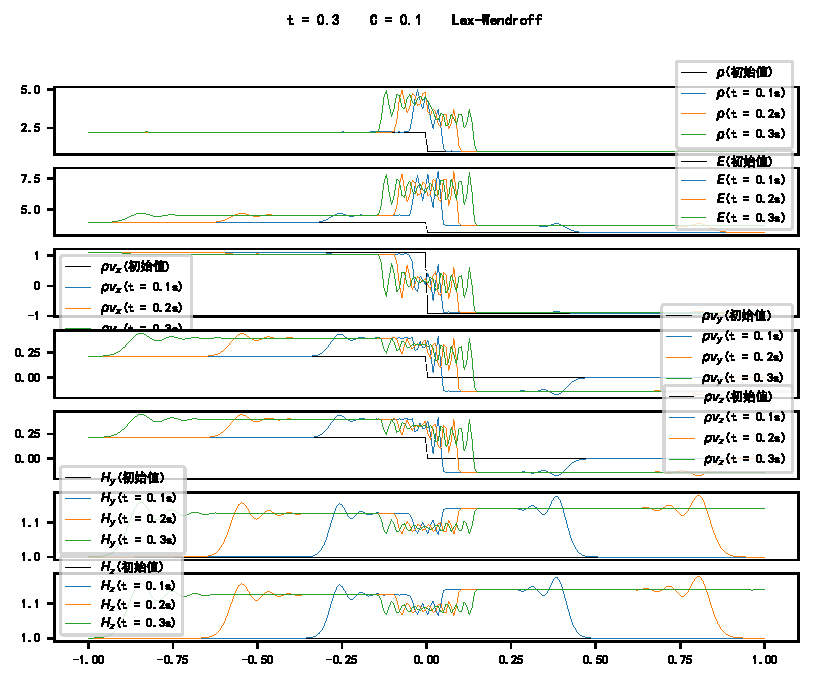
\includegraphics[width=\textwidth]{figures/init2.pdf}
	\caption{Lax-Wendroff 格式计算结果, 网格点数为 261. \textbf{从上到下分别是密度 $\rho$, 能量 $E$ ,质量流 $\rho v_x, \rho v_y, \rho v_z$ 和磁场 $H_y, H_z$。}
	其中点线是初值, 虚线 (上面的数据点用符号 $\circ$ 标注) 是 $t=0.14$ 时的数值结果, 实线是对应的真实解.}
	\label{fig:lax_wendroff2}
\end{figure}

\begin{figure}[htpb]
	\centering
	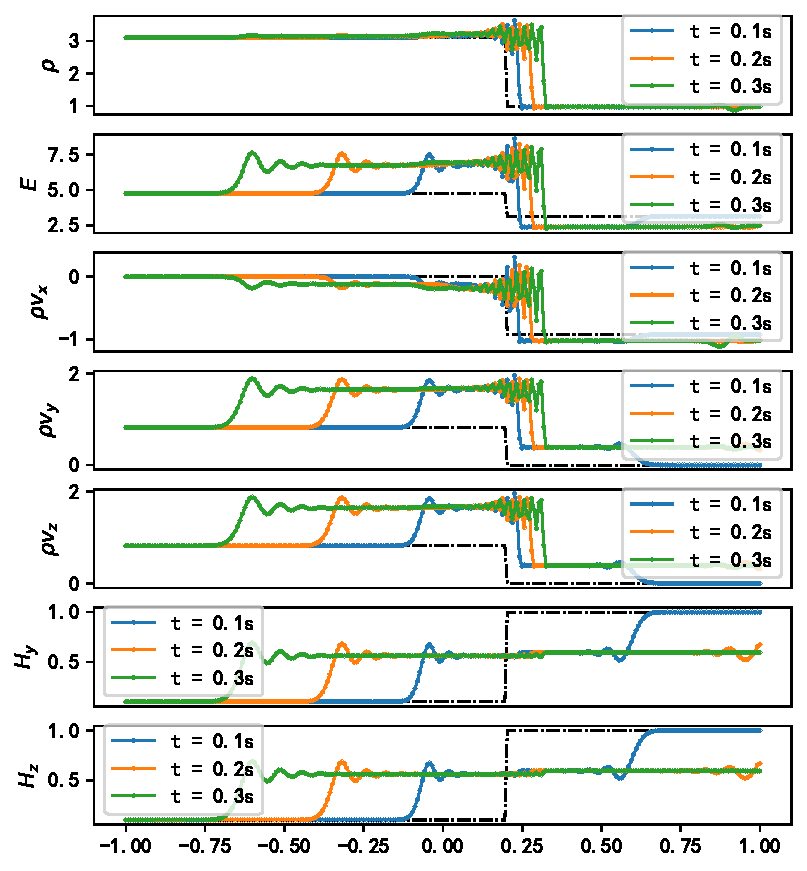
\includegraphics[width=\textwidth]{figures/init4.pdf}
	\caption{Lax-Wendroff 格式计算结果, 网格点数为 261. \textbf{从上到下分别是密度 $\rho$, 能量 $E$ ,质量流 $\rho v_x, \rho v_y, \rho v_z$ 和磁场 $H_y, H_z$。}
	其中点线是初值, 虚线 (上面的数据点用符号 $\circ$ 标注) 是 $t=0.14$ 时的数值结果, 实线是对应的真实解.}
	\label{fig:lax_wendroff4}
\end{figure}

\begin{figure}[htpb]
	\centering
	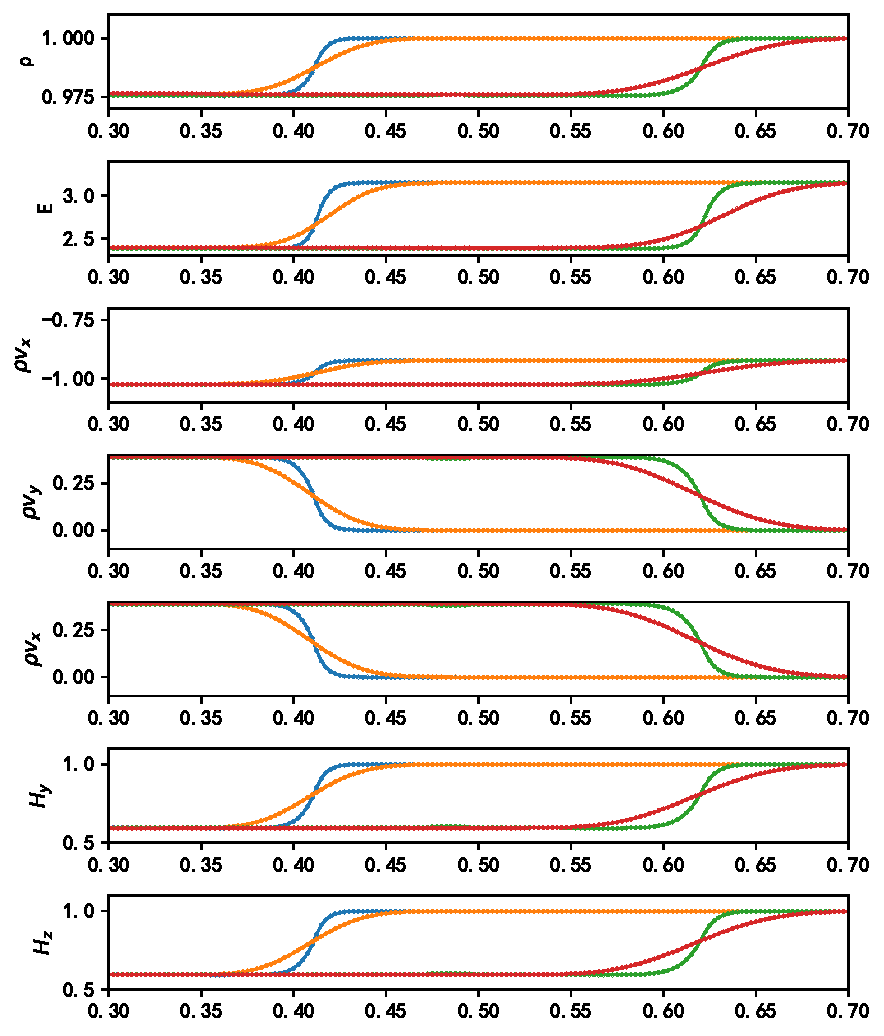
\includegraphics[width=\textwidth]{figures/case1_fast_upwind_TVD.pdf}
	\caption{使用 Upwind 和 TVD 格式计算较弱的慢激波,取 \(x_0 = 0.0,\), 网格点数为 300. \textbf{从上到下分别是密度 $\rho$, 能量 $E$ ,质量流 $\rho v_x, \rho v_y, \rho v_z$ 和磁场 $H_y, H_z$。}
	}%
	\label{fig:upwind_tvd_1}
\end{figure}

\begin{figure}[htpb]
	\centering
	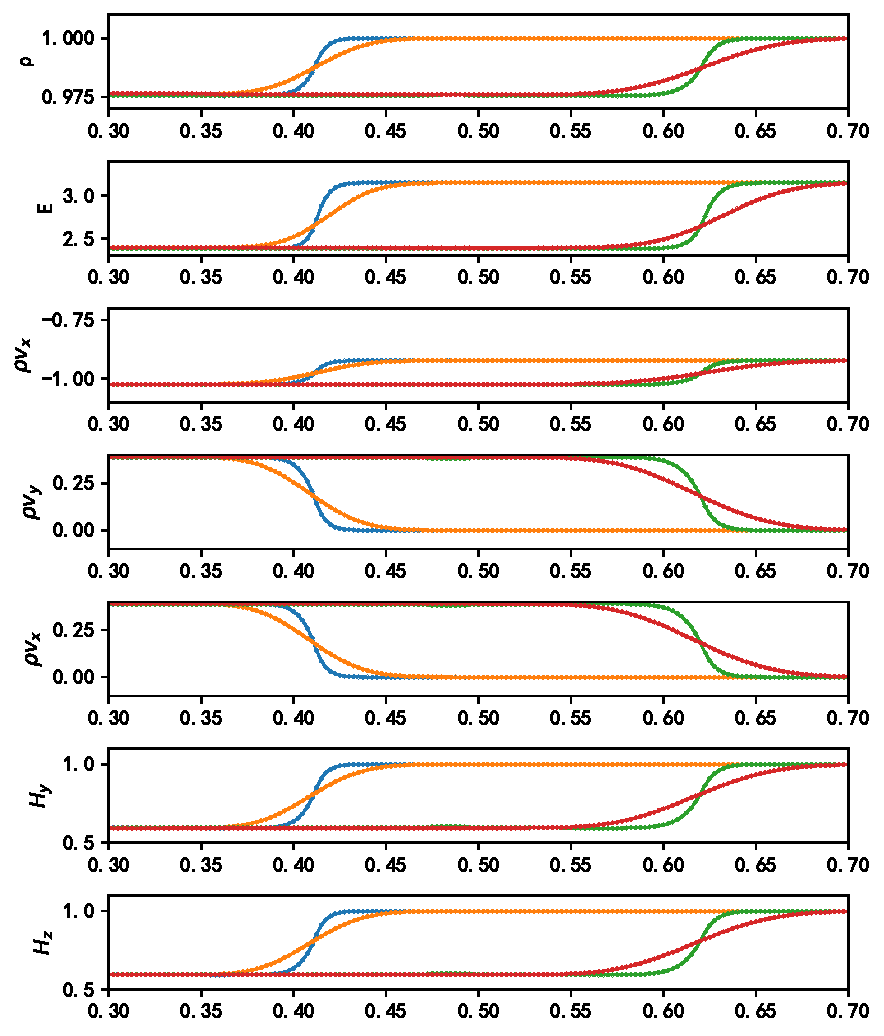
\includegraphics{figures/case3_fast_upwind_TVD.pdf}
	\caption{使用 Upwind 和 TVD 格式计算较弱的慢激波,取 \(x_0 = 0.2,\), 网格点数为 300. \textbf{从上到下分别是密度 $\rho$, 能量 $E$ ,质量流 $\rho v_x, \rho v_y, \rho v_z$ 和磁场 $H_y, H_z$。}
	}%
	\label{fig:upwind_tvd_2}
\end{figure}


\begin{figure}[htpb]
	\centering
	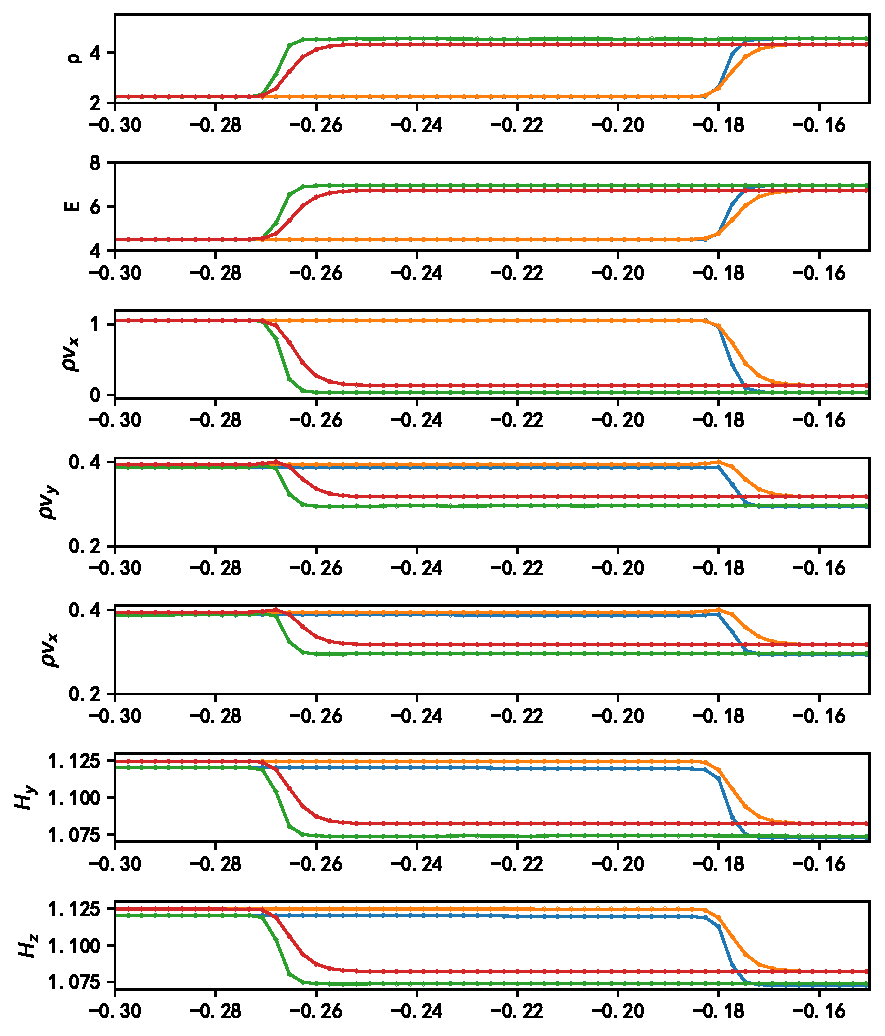
\includegraphics[width=\textwidth]{figures/case1_slow_upwind_TVD.pdf}
	\caption{使用 Upwind 和 TVD 格式计算较弱的慢激波,取 \(x_0 = 0.0,\), 网格点数为 300. \textbf{从上到下分别是密度 $\rho$, 能量 $E$ ,质量流 $\rho v_x, \rho v_y, \rho v_z$ 和磁场 $H_y, H_z$。}
	}%
	\label{fig:upwind_tvd_3}
\end{figure}

\section{其他数值方法尝试与分析}
由于在处理激波时经常出现程序不稳定而崩溃,我们在尝试其他数值方法时试图使用能保持稳定的隐格式。主要使用中间差分的隐格式。
$$
u_j^{n+1} = u_j^n - \frac{\Delta t}{2\Delta x} (F_{j+1}^{n+1} - F_{j-1}^{n+1})
$$
在使用隐格式处理各种不同的方程时,我们遇到如下问题。
\begin{enumerate}
\item
常系数微分方程--可以很容易拆分成三对角矩阵,使用追赶法求解。结果能保证稳定,但是耗散较大。
\item
变系数微分方程--如Burges方程,无法直接拆分成三对角矩阵,但是可以将系数前提,并且系数使用显格式,可以求解,结果稳定,形成的激波间断耗散比较大。
\item
多个特征值的方程组--如第三题的理想气体黎曼问题,三对角矩阵的每一个元素都是一个矩阵,同时使用显格式系数。在随时间迭代时发现数学上无法得到下一时刻的解,需要与迭代法同时使用。
\end{enumerate}
同时,我们在尝试使用迭代法的过程中未能成功用代码求解出稳定的图像出来。因此只能使用TVD等格式模拟较弱的快慢激波。
\section{附件}
附件及附件的说明见 \href{./appendix.txt}{appendix.txt} 

% 以下两行是中文文献国家标准的格式, 如果安装了这两个格式, 建议使用它们
\bibliographystyle{gbt7714-author-year}
% \bibliographystyle{gbt7714-numerical}
%

\bibliography{References}

\end{document}
